\documentclass{beamer}
\usepackage{HECbeamer}
% \usepackage{pgfpages}
% \pgfpagesuselayout{4 on 1}[letterpaper, landscape, border shrink=5mm]
\title[\color{white}{MATH 60604 \S~7e - Test du log rang}]{\texorpdfstring{MATH 60604 \\Modélisation statistique \\ \S~7e - Test du log rang}{MATH 60604 \\ Modélisation statistique \\ \S~7e - Test du log rang}}
\author{}
\institute{HEC Montréal\\
Département de sciences de la décision}
\date{} 

\begin{document}
\frame{\titlepage}
\begin{frame}
 
\frametitle{Comparaison de courbes de survie}
 Les données \code{cancersein} contiennent les résultats d'une étude sur la survie de femmes atteintes du cancer du sein.
\begin{itemize}
\vp \vp
\item \code{temps}: temps avant la mort, ou la fin de l'étude, en mois.
\item \code{mort}: variable indicatrice pour la mort, \code{0} pour les survivantes et \code{1} pour les décédées
\item \code{repimmuno}: réponse immunohistochimique, soit négative (\code{0}) ou positive (\code{1})
\end{itemize}
 On s'intéresse à la question suivante:
\begin{itemize}
\vp \vp
\item Est-ce que les femmes qui répondent positivement à l'examen immunohistochimique ont tendance à survivre moins longtemps que celles qui répondent négativement?
\end{itemize}

\end{frame}

\begin{frame}[fragile]
\frametitle{Comparaison de courbes de survie}
On peut ajuster des courbes de survie différentes par groupe avec l'option \code{strata}.
\vp \vp
\begin{tcolorbox}[colback=white,colframe=hecblue,title=Code \SASlang{} pour le modèle de Kaplan--Meier]
\begin{verbatim}
proc lifetest data=modstat.cancersein method=km;
time temps*mort(0);
strata repimmuno;
run;
\end{verbatim}
\end{tcolorbox}
{\footnotesize 

\SASlang{} va estimer la courbe de survie pour les individus avec une réaction négative (groupe \code{repimmuno=0}) séparément de ceux qui ont une réaction positive (groupe \code{repimmuno=1}).


}
\end{frame}
\begin{frame}[fragile]
\frametitle{Courbes de survie (Kaplan--Meier)}
\begin{center}
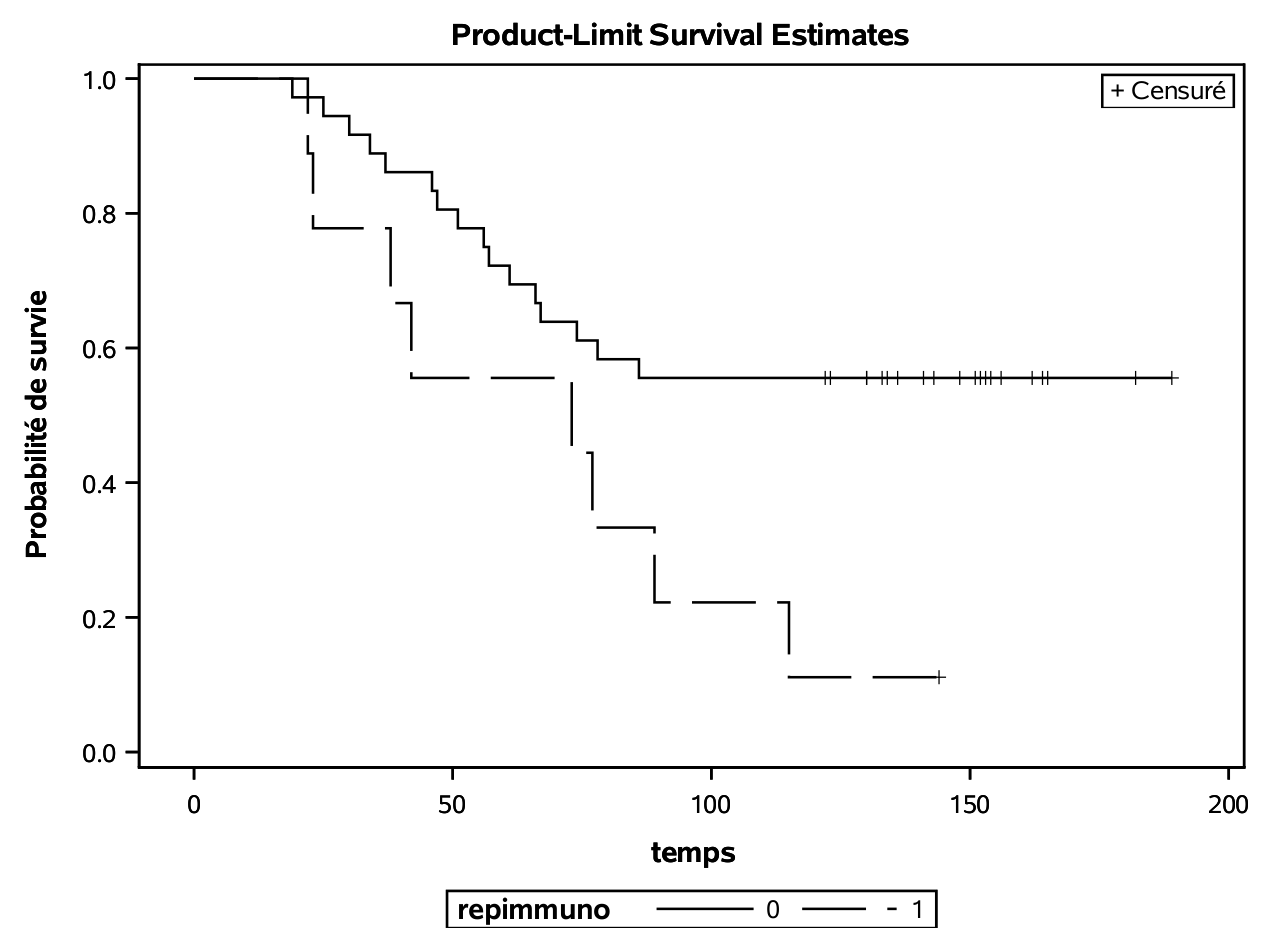
\includegraphics[width = 0.7\textwidth]{img/c7/diapos7e15}
 \end{center}
\end{frame}

\begin{frame}
\frametitle{Comparaison de courbes de survie}
Il semble que les femmes ayant une réaction négative à l'examen (\code{repimmuno=0}) ont un \alert{meilleur} taux de survie que celles qui ont une réaction positive (\code{repimmuno=1}).
\begin{itemize}
% \vp \vp
% \item On peut dire ceci puisque la courbe estimée pour le groupe \code{repimmuno=0}, $\widehat{S}_1(t)$, se situe principalement au-dessus de la courbe estimée pour le groupe \code{repimmuno=1}, $\widehat{S}_2(t)$.
\item Pour la majorité des temps $t$, $\widehat{S}_1(t) > \widehat{S}_2(t)$ et donc ceux avec \code{repimmuno=0} ont une probabilité de survie supérieure à ceux avec \code{repimmuno=1}
\end{itemize}
% \item Mais est-ce que ces courbes sont \emph{significativement} différentes?
% \begin{itemize}
% \vp \vp
Est-ce que la fonction de survie est significativement différente dans les deux groupes \code{repimmuno=0} et \code{repimmuno=1}?
% \begin{itemize}
% \vp \vp
% \item[] $\Hy_0$: les courbes de survie sont les mêmes dans les deux groupes 
% \item[] $\Hy_1$: les courbes de survie sont différentes dans les deux groupes
% \end{itemize}
% \end{itemize}
% \item De façon plus formelle, on est intéressé à tester
\begin{itemize}
\vp \vp
\item[] $\Hy_0: S_0(t) = S_1(t)$ pour tout $t$,
\item[] $\Hy_1: S_0(t) \neq S_1(t)$ pour au moins une valeur de $t$.
\end{itemize}
% \end{itemize}
\end{frame}

\begin{frame}[fragile]
\frametitle{Test du log rang}
 Considérons un modèle à risques proportionnels de Cox avec fonction de risque
 \begin{align} 
  h(t) = h_0(t)\exp(\beta \code{repimmuno}). \tag{$\star$} \label{lograngtest}
 \end{align}
\bi 
\item 
L'hypothèse nulle pour l'égalité des fonctions de survie est équivalente à $\Hy_0: \beta=0$. 
\item La statistique du score permet de tester cette hypothèse sans ajuster le modèle.
\bi \item On recouvre l'estimateur de Kaplan--Meier de la fonction de survie si $\beta=0$.
\ei
\item Il suffit de calculer le gradient et la hessienne du modèle décrit par \eqref{lograngtest} et l'évaluer en $\beta=0$. 
\bi
\item Ce sont des fonctions simples du nombre de personnes à risque dans chaque groupe aux temps $t_i$.
\ei 
\ei
\end{frame}
% \begin{frame}
%  \frametitle{Statistique du log rang}
%  
%  
%  
%  Pour deux groupes, s'il n'y a pas de doublons, on obtient
%  \begin{align*}
% \left.U(\beta)\right|_{\beta=0}& = \sum_{i: \delta_i=1} \left(f_i - \frac{m_{i1}}{m_{i0}+m_{i1}}\right), 
% \\\left.j(\beta)\right|_{\beta=0}&= \sum_{i: \delta_i=1} \frac{m_{i0}m_{i1}}{(m_{i0} + m_{i1})^2}
%  \end{align*}
% où 
% \bi \item $f_j$ vaut un si l'individu $i$ expérience l'événement au temps $t_i$ et 
% \item $m_{ij}$ est le nombre d'individus à risque au temps $t_i$ pour le groupe $j$.
% \ei
% \end{frame}
\begin{frame}[fragile]
\frametitle{Ajustement du modèle à risques proportionnels}
\begin{tcolorbox}[colback=white,colframe=hecblue, title=Code \SASlang{} pour le modèle de risques proportionnels]
\begin{verbatim}
proc phreg data=modstat.cancersein;
model temps*mort(0) = repimmuno;
run;
\end{verbatim}
\end{tcolorbox}
\begin{center}
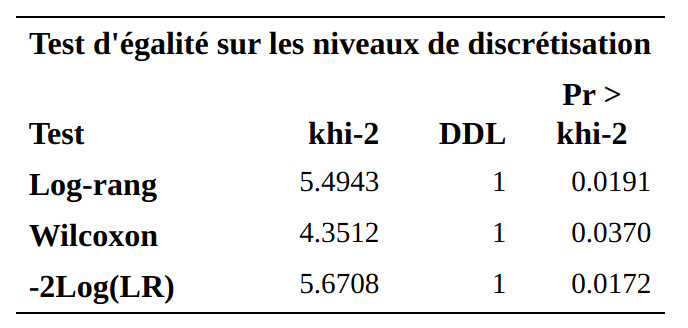
\includegraphics[width = 0.5\textwidth]{img/c7/diapos7e16}
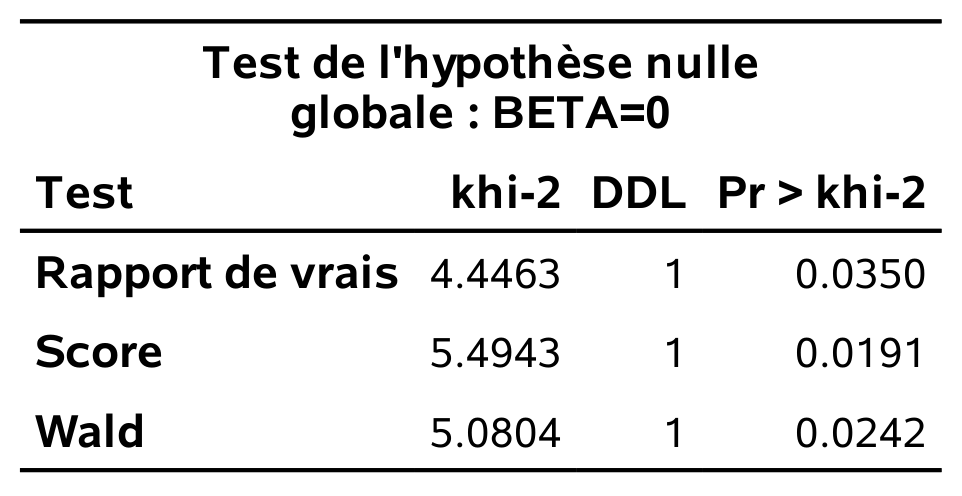
\includegraphics[width = 0.45\textwidth]{img/c7/diapos7e17}
\end{center}
{\footnotesize 

Le test du log rang est aussi présenté par défaut dans la sortie \SASlang{} de la procédure \code{lifetest} (gauche).

}
\end{frame}

\begin{frame}
\frametitle{Test du log rang}
\bi 
\item Sous $\Hy_0: \beta=0$, la loi nulle de la statistique de score est approximativement $\chi^2_1$.
\item La valeur-$p$  est $0.0191$: on rejette $\Hy_0$ à niveau $5\%$ et on conclut que les fonctions de survie sont significativement différentes pour les femmes avec des réactions négatives / positives à l'examen immunohistochimique. 
\item On peut généraliser le test du log rang en utilisant un modèle de Cox qui n'inclut qu'une variable catégorielle à $k$ niveaux
\bi \item la loi nulle de la statistique du test de score sera $\chi^2_{k-1}$.
\ei
\ei 
\end{frame}


% \begin{frame}
% \frametitle{Comparaison de courbes de survie}
% Quelques remarques...
% \vp \vp \vp \vp \vp
% \begin{itemize}
% \item Notez qu'il existe une extension du test qui permet de comparer les fonctions de survie pour plusieurs groupes:
% \begin{itemize}
% \vp \vp
% \item[] $\Hy_0: S_1(t) = S_2(t) = \cdots = S_K(t)$
% \item[] $\Hy_1:$ au moins deux des fonctions sont différentes pour au moins un $t$ 
% \item Dans le cas du test de log rang, la distribution de la statistique de test sous $\Hy_0$ sera $\chi^2_{k-1}$.
% \end{itemize}
% \vp \vp \vp \vp \vp
% % 
% % \item Notez: le test Wilcoxon est un alternatif au test de log rang, qui a une forme très similaire au test de log rang. Le $-2LL$ montre les résultats pour un test de rapport de vraisemblance qui suppose que les temps de survie suivent une loi exponentielle. 
% \end{itemize}
% \end{frame}
\end{document}
